
\documentclass[11pt,a4paper,openany]{report}
\usepackage[T1]{fontenc}
\usepackage[utf8]{inputenc}
\usepackage{lmodern}
\usepackage{microtype}
\usepackage{amsmath,amssymb,amsthm,mathtools,bm}
\usepackage{booktabs,array,longtable,tabularx}
\usepackage{xcolor}
\usepackage[margin=22mm,headheight=23pt]{geometry}
\usepackage{enumitem}
\usepackage{fancyhdr}
\usepackage{fancyvrb}
\usepackage{graphicx}
\usepackage{url}
\usepackage{xurl}
\usepackage{hyperref}
\definecolor{finblue}{HTML}{1F5A99}
\definecolor{fingreen}{HTML}{19733A}
\definecolor{finorange}{HTML}{D55E00}
\definecolor{finred}{HTML}{A61B1B}
\definecolor{finviolet}{HTML}{6A3D9A}
\definecolor{fingray}{HTML}{4D4D4D}

\hypersetup{
  unicode=true,
  colorlinks=true,
  linkcolor=finblue,
  citecolor=fingreen,
  urlcolor=finblue,
  pdftitle={FIN Research Programs P365--P378},
  pdfauthor={Krzysztof Żuchowski},
  pdfsubject={Exact certificate diversity, adaptive discrimination, operational resource semantics, and the universality boundary},
  pdfkeywords={FIN, exact certificate, Krawczyk method, Bernstein certificate, radial kernel naturality, adaptive quantum discrimination, data processing, outer function, operational resource theory}
}
\pagestyle{fancy}
\fancyhf{}
\fancyhead[L]{\small FIN Programs P365--P378}
\fancyhead[R]{\small Release 10.32}
\fancyfoot[C]{\thepage}

\setlength{\parindent}{0pt}
\setlength{\parskip}{0.55em}
\setlist{nosep,leftmargin=2em}
\setcounter{tocdepth}{2}
\setcounter{secnumdepth}{3}
\emergencystretch=3em
\newcommand{\one}{\bm 1}
\newcommand{\C}{\mathbb C}
\newcommand{\R}{\mathbb R}
\newcommand{\Z}{\mathbb Z}
\newcommand{\statusProven}{\textcolor{fingreen}{[Proven]}}
\newcommand{\statusStrong}{\textcolor{finblue}{[Strong evidence]}}
\newcommand{\statusModerate}{\textcolor{finviolet}{[Moderate evidence]}}
\newcommand{\statusWeak}{\textcolor{fingray}{[Weak evidence]}}
\newcommand{\statusSpeculative}{\textcolor{finorange}{[Speculative]}}
\newcommand{\statusRefuted}{\textcolor{finred}{[Refuted]}}

\begin{document}
\hypersetup{pageanchor=false}
\begin{titlepage}
\centering
\vspace*{7mm}
{\Large\bfseries FIN --- Release 10.32\par}
\vspace{9mm}
{\Huge\bfseries Research Programs P365--P378\par}
\vspace{6mm}
{\Large Exact certificate diversity, adaptive discrimination,\\
operational resource semantics, and the universality boundary\par}
\vspace{13mm}
{\Large Krzysztof \.Zuchowski\par}
\vspace{2mm}
{\normalsize Independent Researcher --- Fractal Information Theory Project\par}
\vspace{2mm}
{\normalsize ORCID:
\href{https://orcid.org/0009-0002-0909-3613}{0009-0002-0909-3613}\par}
\vspace{7mm}
{\large 31 July 2026\par}
{\normalsize Publication --- Preprint; Version 1.0.0\par}
\vfill
\begin{minipage}{0.92\textwidth}
\small
\textbf{Tightened oscillatory resource.}
\[
0.7072784585518420
\leq\mathcal N_{\rm osc}
\leq0.7073534683998260.
\]

\textbf{Ideal adaptive discrimination, first perfect branch.}
\[
\frac12\left\|
\mathcal U_{\rm strict}^{\otimes n}
-\mathcal U_{\rm legacy}^{\otimes n}
\right\|_{\diamond}
=
\sin\!\left(\frac{nt\Delta}{2}\right),
\qquad
0\leq t\leq\frac{\pi}{n\Delta}.
\]

The signed quantity is a classical representation cost. The channel theorem
is restricted to the declared commuting, ideal-unitary comparison and its
first perfect time. No selector, dimensional standard, laboratory
realization, physical role transfer, Standard Model, gravity, or
Theory-of-Everything closure is claimed.

\medskip
\textbf{Repository.}
\url{https://github.com/hyconiek/Fractal-Nadsoliton-Theory}

\textbf{License.} CC BY 4.0.
\end{minipage}
\vfill
\end{titlepage}
\hypersetup{pageanchor=true}
\pagenumbering{roman}
\chapter*{Publication statement}
\addcontentsline{toc}{chapter}{Publication statement}
This monograph reports every executed Program P365--P378 and recommends
Programs P379--P393. Exact proof, high-precision computation, synthetic
apparatus modelling, conditional operational semantics, and absent external
evidence are kept distinct. The legacy/strict split and all current
strict-core guardrails remain binding.

\tableofcontents
\clearpage
\pagenumbering{arabic}

\chapter*{Confidence convention}
\addcontentsline{toc}{chapter}{Confidence convention}

\begin{center}
\begingroup\small
\setlength{\tabcolsep}{2.5pt}
\renewcommand{\arraystretch}{1.16}
\begin{longtable}{@{}p{0.420\textwidth}p{0.420\textwidth}@{}}
\toprule
\textbf{Label} & \textbf{Meaning} \\
\midrule
\endhead
\textbf{\statusProven{}} & Exact mathematical proof, exact rational computation, exhaustive finite classification, or compiled structural formal theorem \\
\textbf{\statusStrong{}} & Reproducible high-precision computation with explicit residual and robustness boundary \\
\textbf{\statusModerate{}} & Model-dependent synthetic or local result with stated assumptions \\
\textbf{[Conditional]} & Result requiring named encodings, axioms, standards, or operational identifications \\
\textbf{\statusRefuted{}} & The declared proposition fails in its stated class \\
\textbf{[Blocked by external evidence]} & Independent data, hardware, calibration, standards, custody, or unblinding is required \\
\bottomrule
\end{longtable}
\endgroup
\end{center}

\chapter{Scientific scope and guardrails}

\section{Kernel split}

The legacy intermediate kernel remains

\[
K_{\mathrm{legacy,ont}}(d)=
4\ln2\,
\frac{\cos(\pi d/4+\pi/6)}{1+0.01d},
\]

whereas the strict working kernel is

\[
K_{\mathrm{strict,gate}}(d)=
\frac{\cos((743/4000)d+13/80)}{1+d^{9/5}}.
\]

No identity between these functions is assumed. The scale \(\gamma=0.13044237640961015\) used in P371 is the frozen operational comparison scale from P328/\allowbreak{}P343, not a bridge-completion or physical role-transfer theorem.

\section{Ontology}

The repository order remains

\[
\text{nadsoliton}
\longrightarrow
\text{light}
\longrightarrow
\text{matter}
\longrightarrow
\text{emergent observer}.
\]

The nadsoliton is the primordial information in a solitonic state, not an object above a second informational substrate. None of the proofs below uses this ontology as a mathematical premise.

\section{Preserved open boundaries}

This report does not close:

\begin{itemize}
\item 
QW-2191 or the non-premise selector;

\item 
the legacy-to-strict completion;

\item 
legacy physical-role transfer;

\item 
an internal length, time, action, energy, or mass standard;

\item 
a laboratory realization functor;

\item 
a unit-bearing nonproxy total action;

\item 
Standard Model or gravity generation;

\item 
Theory-of-Everything closure.

\end{itemize}

\chapter{Executive results}

\begin{center}
\begingroup\small
\setlength{\tabcolsep}{2.5pt}
\renewcommand{\arraystretch}{1.16}
\begin{longtable}{@{}p{0.120\textwidth}p{0.420\textwidth}p{0.320\textwidth}@{}}
\toprule
\textbf{Program} & \textbf{Result} & \textbf{Status} \\
\midrule
\endhead
P365 & Independent exact checker reproduces P351/\allowbreak{}P352 identities & \statusProven{} /\allowbreak{} proof-assistant arithmetic still blocked \\
P366 & Oscillatory enclosure tightened to \([0.7072784586,0.7073534684]\) & \statusProven{} \\
P367 & No independent QW hold-out admitted & [Blocked] \\
P368 & Maximal \(k\)-distance quotient category; exhaustive small-graph classification & \statusProven{} \\
P369 & Complex transfer locally full-rank; intensity calibration ill-conditioned & \statusModerate{} \\
P370 & No calibrated photonic pilot admitted & [Blocked] \\
P371 & Full ideal adaptive optimum through the first perfect time & \statusProven{} \\
P372 & No traceable clock anchor admitted & [Blocked] \\
P373 & Five operational data-processing monotones & \statusProven{} /\allowbreak{} [Conditional] FIN encoding \\
P374 & Noncanonical outer analytic extension family & \statusProven{} \\
P375 & No conditional EW blind-test bundle admitted & [Blocked] \\
P376 & No dimensional standards bundle admitted & [Blocked] \\
P377 & FORC resource syntax free; unique operational universality false & \statusProven{} /\allowbreak{} \statusRefuted{} \\
P378 & No reservoir tomography bundle admitted & [Blocked] \\
\bottomrule
\end{longtable}
\endgroup
\end{center}

\chapter{P365 --- independent checking is not self-replay}

\section{Checker separation}

The P365 checker:

\begin{itemize}
\item 
imports no FIN research module;

\item 
reimplements rational intervals;

\item 
reimplements matrix inversion over \(\mathbb Q\);

\item 
reimplements Krawczyk inclusion;

\item 
reimplements fifth-root brackets;

\item 
reimplements Taylor/\allowbreak{}Lagrange cosine intervals;

\item 
reimplements Bernstein conversion and subdivision;

\item 
recomputes the exact Vandermonde inverse;

\item 
compares byte-level rational identities with archived certificates.

\end{itemize}

\section{Results}

The checker reproduces:

\begin{center}
\begingroup\small
\setlength{\tabcolsep}{2.5pt}
\renewcommand{\arraystretch}{1.16}
\begin{longtable}{@{}p{0.420\textwidth}p{0.420\textwidth}@{}}
\toprule
\textbf{Component} & \textbf{Checks} \\
\midrule
\endhead
P351 Krawczyk interval endpoints & 12 \\
P352 safe dual coefficients & 12 \\
P352 weight interval endpoints & 24 \\
P352 Bernstein feasibility & passed \\
P352 twelve weight signs & passed \\
\bottomrule
\end{longtable}
\endgroup
\end{center}

All checks pass.

\section{Confidence boundary}

\textbf{\statusProven{}} A second implementation using exact arbitrary-precision arithmetic accepts the certificates.

\textbf{[Blocked]} The large arithmetic is not yet reflected through a Lean or Coq kernel. The compiled Lean file proves structural implications only.

This distinction matters. Independent implementation reduces the risk of a shared code-path error; proof-assistant reflection would additionally reduce the trusted computing base.

\chapter{P366 --- a tighter seven-atom oscillatory certificate}

\section{Exact dual refinement}

P352 used 4096 rational Bernstein subintervals. P366 uses a depth-fourteen dyadic de Casteljau tree:

\[
2^{14}=16\,384
\]

subintervals.

For the rational degree-eleven dual candidate \(p_{\mathrm{raw}}\), exact Bernstein extrema \(L,U\) define

\[
p_{\mathrm{safe}}(x)=
\frac{p_{\mathrm{raw}}(x)-U}{U-L}.
\]

The same dyadic tree proves

\[
-1\leq p_{\mathrm{safe}}(x)\leq0
\qquad(0\leq x\leq1).
\]

Exact oscillatory moment intervals then give

\[
\mathcal N_{\mathrm{osc}}
\geq0.7072784585518420.
\]

\section{Seven-atom primal}

The first node is fixed exactly at

\[
r_1=
\frac{19826532267005523}{10^{18}}.
\]

The remaining unknowns are:

\begin{itemize}
\item 
five interior nodes;

\item 
seven weights.

\end{itemize}

All twelve moment equations are included. The exact rational Krawczyk image is strictly contained in a radius-\(10^{-20}\) box for all twelve variables. The certified sign pattern is

\[
(-,+,+,+,+,-,+).
\]

The corresponding feasible negative mass satisfies

\[
\mathcal N_{\mathrm{osc}}
\leq0.7073534683998260.
\]

\section{Result}

\[
\boxed{
0.7072784585518420
\leq
\mathcal N_{\mathrm{osc}}
\leq
0.7073534683998260
}.
\]

Compared with P352:

\begin{itemize}
\item 
the lower endpoint improves by \(2.3323561\times10^{-7}\);

\item 
the upper endpoint improves by \(6.5064864\times10^{-6}\);

\item 
the width decreases by \(8.244\%\).

\end{itemize}

\section{Interpretation boundary}

This is the minimum negative part of a signed scalar representing measure in the declared truncated Hausdorff problem. It is not automatically:

\begin{itemize}
\item 
quantum quasiprobability;

\item 
negative information;

\item 
dissipated entropy;

\item 
negative energy;

\item 
an adaptive feedback strength;

\item 
a physical coupling.

\end{itemize}

\begin{figure}[htbp]
\centering
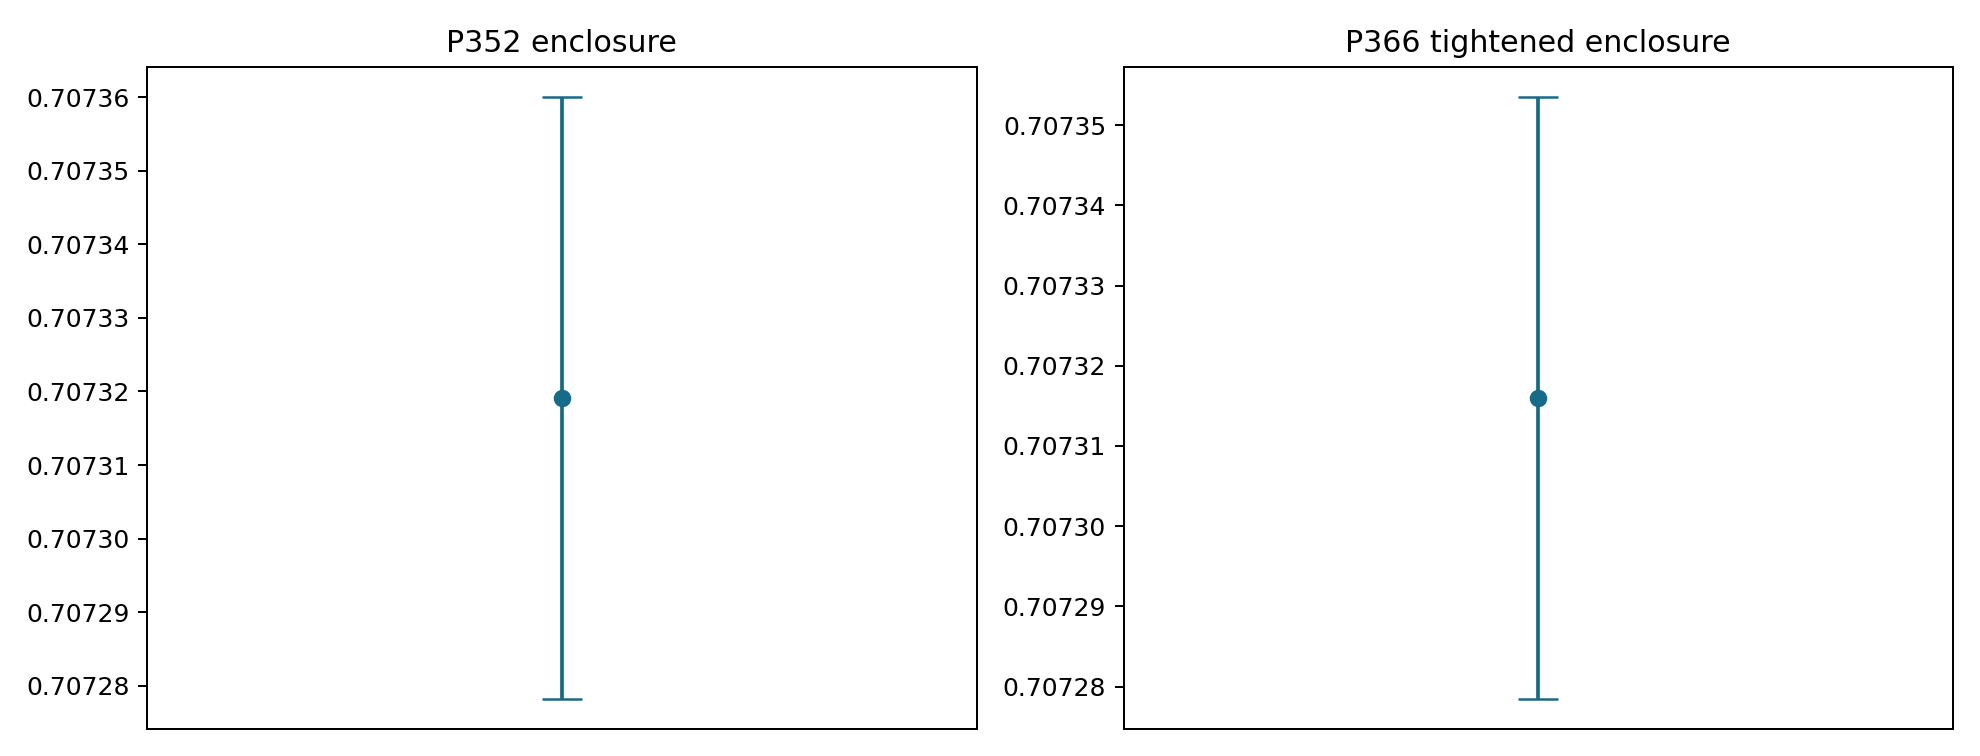
\includegraphics[width=0.97\textwidth]{FIN_Programs_365_378_Figures/p365_p366_certificate_tightening.png}
\caption{Independent exact certificate checking and the tightened oscillatory signed-moment enclosure.}
\end{figure}

\chapter{P367 --- external hold-out gate}

No manifest satisfies the independent provider/\allowbreak{}registrar/\allowbreak{}analyst, freeze-hash, and one-shot unblinding contract.

\textbf{[Blocked by external evidence]}

The continuous QW refreeze remains in-sample. Its numerical stability cannot be promoted to an empirical prediction.

\chapter{P368 --- the maximal radial naturality category}

\section{Exact categorical definition}

Let \(G,H\) be finite metric carriers and \(k\) a radial law. A map \(f:G\to H\) preserves the radial kernel exactly when

\[
k(d_H(f(x),f(y)))
=
k(d_G(x,y))
\]

for all \(x,y\).

Define the distance equivalence relation

\[
d\sim_k e
\quad\Longleftrightarrow\quad
k(d)=k(e).
\]

Then \(f\) is kernel-preserving precisely when it preserves the \(\sim_k\)-class of every pairwise distance.

These maps contain identities and are closed under composition. They form the maximal category on which the radial kernel is strictly natural.

\section{Injective-distance corollary}

If \(k\) is injective on the attainable distance set, then

\[
k(d_H(fx,fy))=k(d_G(x,y))
\quad\Longleftrightarrow\quad
d_H(fx,fy)=d_G(x,y).
\]

Thus the maximal naturality category reduces to isometric embeddings.

\section{Exact small-distance certificate}

Exact rational intervals for

\[
k_{\mathrm{strict}}(1),\ldots,k_{\mathrm{strict}}(4)
\]

are pairwise disjoint. Consequently the strict kernel is injective on the distance sets of connected graphs with at most five vertices.

\section{Exhaustive atlas}

The finite audit covers all thirty connected unlabeled graphs with two to five vertices.

\begin{center}
\begingroup\small
\setlength{\tabcolsep}{2.5pt}
\renewcommand{\arraystretch}{1.16}
\begin{longtable}{@{}p{0.420\textwidth}p{0.420\textwidth}@{}}
\toprule
\textbf{Quantity} & \textbf{Count} \\
\midrule
\endhead
Graph pairs admitting at least one homomorphism & 607 \\
Graph homomorphisms & 77,130 \\
Isometric embeddings & 1,664 \\
Strict-kernel-preserving maps & 1,664 \\
Classification mismatches & 0 \\
\bottomrule
\end{longtable}
\endgroup
\end{center}

\section{Boundary}

No global theorem says the oscillatory law is injective for every integer distance. Larger carriers must use the \(k\)-distance quotient unless further distance intervals are certified.

This result classifies carrier transport. It does not construct a legacy-to-strict completion law.

\chapter{P369--P370 --- component losses and the photonic boundary}

\section{Model}

The ideal twelve-mode unitary has 66 Givens components. P369 assigns:

\begin{itemize}
\item 
one logarithmic insertion-loss parameter per component;

\item 
one phase-error parameter per component.

\end{itemize}

The unknown parameter count is therefore

\[
2\times66=132.
\]

\section{Local identifiability}

At the ideal point, finite-difference Jacobians give:

\begin{center}
\begingroup\small
\setlength{\tabcolsep}{2.5pt}
\renewcommand{\arraystretch}{1.16}
\begin{longtable}{@{}p{0.326\textwidth}p{0.232\textwidth}p{0.301\textwidth}@{}}
\toprule
\textbf{Observation} & \textbf{Effective rank} & \textbf{Condition number} \\
\midrule
\endhead
Complex transfer matrix & 132 & \(1.94\times10^2\) \\
Intensities \(|T_{ij}|^2\) & 123 & \(5.66\times10^7\) \\
Conditional intensities & 118 & \(8.32\times10^7\) \\
\bottomrule
\end{longtable}
\endgroup
\end{center}

The threshold is \(10^{-8}\) relative to the largest singular value.

\textbf{\statusModerate{}}

Complex transfer tomography is locally informative for all declared parameters. Intensity-only observations possess practically unresolved directions and severe conditioning.

\section{Correlated-error stress test}

The synthetic model varies:

\begin{itemize}
\item 
loss from \(0.001\) to \(0.01\) dB per component;

\item 
phase noise from \(10^{-4}\) to \(10^{-3}\) radians;

\item 
phase AR(1) correlation \(0\) or \(0.8\);

\item 
64 runs per setting.

\end{itemize}

The worst tested setting has

\[
\mathrm{TV}_{95}=0.0051152391,
\]

and fifth-percentile minimum click probability

\[
0.9606933924.
\]

\section{What this changes experimentally}

A credible photonic pilot must freeze a complex transfer calibration, not only vertex intensity images. It must also report:

\begin{itemize}
\item 
phase-reference stability;

\item 
source coherence and multiphoton contamination;

\item 
detector efficiency and crosstalk;

\item 
raw event timestamps;

\item 
calibration uncertainty;

\item 
independent custody.

\end{itemize}

P370 finds no admitted physical bundle.

\textbf{[Blocked by external evidence]}

\begin{figure}[htbp]
\centering
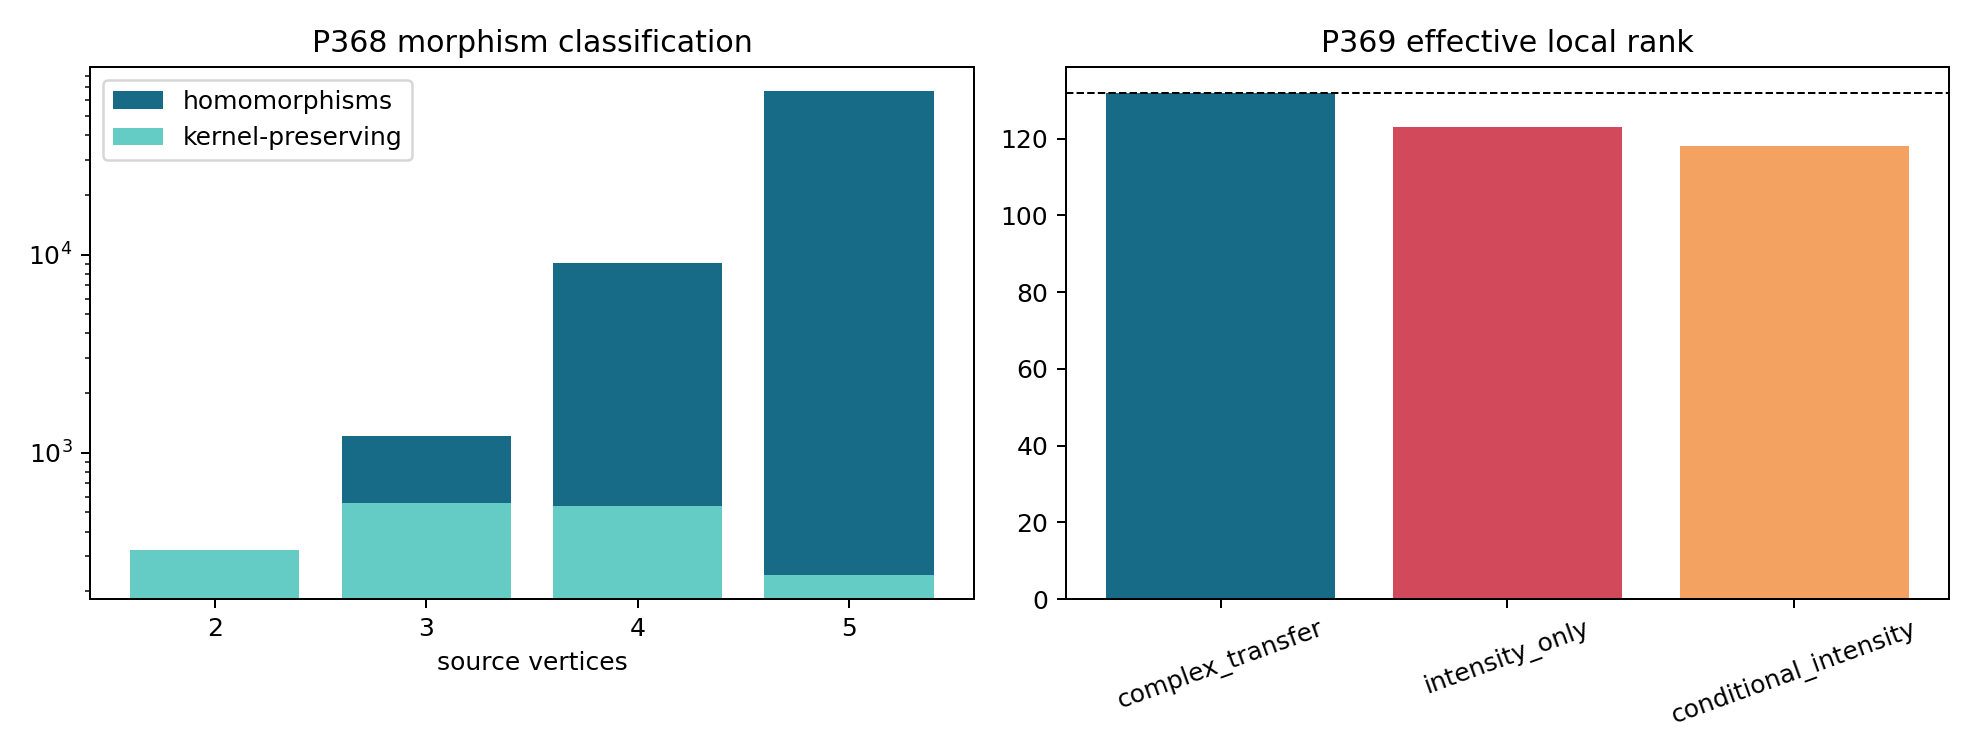
\includegraphics[width=0.97\textwidth]{FIN_Programs_365_378_Figures/p368_p369_naturality_identifiability.png}
\caption{The maximal radial-kernel naturality category and component-level photonic calibration identifiability.}
\end{figure}

\chapter{P371 --- exact adaptive-angle theorem}

\section{Relative generator}

At the frozen comparison scale \(\gamma\), define

\[
D=\gamma A_{\mathrm{legacy}}-A_{\mathrm{strict}}.
\]

The two circulant generators commute to numerical norm

\[
4.22\times10^{-15}.
\]

Their relative unitary is therefore

\[
U_{\mathrm{strict}}(t)^\dagger
U_{\mathrm{legacy}}(t)
=e^{-itD}.
\]

Let

\[
\Delta=
\lambda_{\max}(D)-\lambda_{\min}(D)
=4.365523996749653.
\]

\section{Adaptive upper bound}

Consider arbitrary coherent memory, ancillas, and common adaptive controls. Before an oracle call, let the two hypothesis branches have Fubini--Study angle \(\Theta\). Applying different unitary hypotheses can add at most

\[
\frac{t\Delta}{2}
\]

to the angle. Common controls preserve the angle. By induction and the triangle inequality,

\[
\Theta_n\leq\frac{nt\Delta}{2}.
\]

For pure output branches, the half trace distance is bounded by

\[
\sin\Theta_n.
\]

This gives an unrestricted adaptive upper bound.

\section{Parallel lower bound}

Let \(|\lambda_{\min}\rangle\) and \(|\lambda_{\max}\rangle\) be extremal eigenvectors of \(D\). A parallel \(n\)-use superposition of the two tensor extremal modes has overlap

\[
\cos\!\left(\frac{nt\Delta}{2}\right).
\]

It therefore attains half trace distance

\[
\sin\!\left(\frac{nt\Delta}{2}\right).
\]

The adaptive upper bound and parallel lower bound coincide.

\section{Theorem}

For

\[
0\leq t\leq\frac{\pi}{n\Delta},
\]

the unrestricted adaptive optimum is

\[
\boxed{
D_n(t)=
\sin\!\left(\frac{nt\Delta}{2}\right)
}.
\]

At

\[
t_n^*=\frac{\pi}{n\Delta},
\]

the two channels are perfectly distinguishable.

\begin{center}
\begingroup\small
\setlength{\tabcolsep}{2.5pt}
\renewcommand{\arraystretch}{1.16}
\begin{longtable}{@{}p{0.420\textwidth}p{0.420\textwidth}@{}}
\toprule
\textbf{Uses \(n\)} & \textbf{\(t_n^*\)} \\
\midrule
\endhead
1 & 0.7196370140053893 \\
2 & 0.3598185070026946 \\
3 & 0.2398790046684631 \\
4 & 0.1799092535013473 \\
\bottomrule
\end{longtable}
\endgroup
\end{center}

The offsets between these values and the earlier P343 sampled grid are all below \(3.63\times10^{-4}\).

\section{Scope}

The theorem solves the ideal commuting unitary pair through the first perfect-discrimination time. It assumes:

\begin{itemize}
\item 
identical calibrated time per use;

\item 
the frozen comparison scale;

\item 
lossless unitary calls;

\item 
arbitrary coherent memory and preparation;

\item 
unrestricted final measurement.

\end{itemize}

It does not solve:

\begin{itemize}
\item 
lossy or dephasing channels;

\item 
uncertain or nonlinear clocks;

\item 
limited ancilla dimensions;

\item 
imperfect instruments;

\item 
the global post-threshold revival structure.

\end{itemize}

\begin{figure}[htbp]
\centering
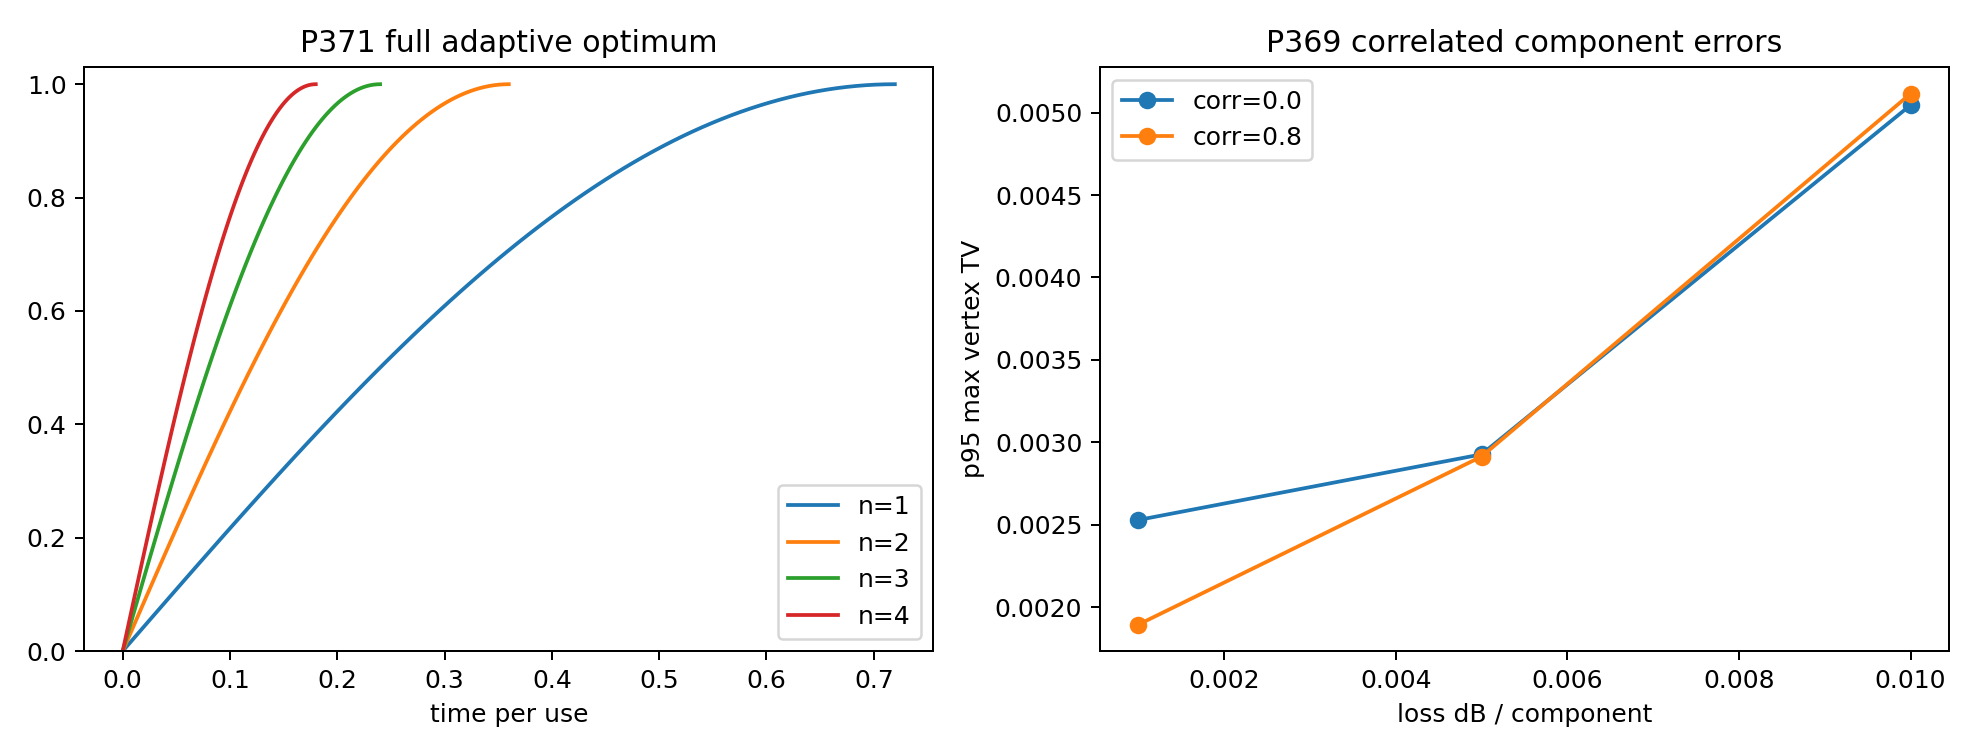
\includegraphics[width=0.97\textwidth]{FIN_Programs_365_378_Figures/p369_p371_loss_comb.png}
\caption{Synthetic component-loss sensitivity and the exact ideal adaptive discrimination law through the first perfect time.}
\end{figure}

\chapter{P372 --- the clock remains external}

P358 proved an equispaced minimax design after a dimensional anchor is supplied. P372 searches for a manifest containing:

\begin{itemize}
\item 
traceable clock-standard hash;

\item 
calibration-record hash;

\item 
provider, registrar, and analyst;

\item 
freeze timestamp;

\item 
unblinding authorization.

\end{itemize}

No admissible package is present.

\textbf{[Blocked by external evidence]}

P371's analytic time parameter is therefore dimensionless repository time, not a calibrated laboratory second.

\chapter{P373 --- operational semantics for five resources}

\section{Signed-path resource}

For a signed measure of fixed total mass,

\[
\mathcal N(\mu)=\mu^-(X)
\]

contracts under positive mass-preserving Markov pushforwards.

\section{Phase resource}

For a density operator,

\[
C_{l_1}(\rho)=
\sum_{i\ne j}|\rho_{ij}|
\]

contracts under the declared dephasing channel.

This is an operational coherence resource. It is not identical to the number-theoretic label "non-torsion phase" without an explicit encoding.

\section{Orientation resource}

For a distribution \(p\) on \(\mathbb Z_{12}\) and reflection \(R\), define

\[
A_R(p)=\frac12\|p-Rp\|_1.
\]

Reflection-covariant Markov convolution commutes with \(R\) and contracts total variation, so

\[
A_R(Tp)\leq A_R(p).
\]

This measures an already prepared orientation asymmetry. It does not source the missing strict selector.

\section{Scale resource}

For a parametric distribution \(p_\theta\), classical Fisher information

\[
I(\theta)=
\sum_x
\frac{(\partial_\theta p_\theta(x))^2}{p_\theta(x)}
\]

contracts under a parameter-independent Markov coarse graining.

This quantifies information about an existing scale parameter. It does not create a dimensional standard.

\section{Cross-law resource}

For a joint distribution,

\[
I(X:Y)=
D_{\mathrm{KL}}(p_{XY}\|p_Xp_Y)
\]

contracts under local stochastic channels.

It measures established correlation and does not derive an independent legacy-to-strict completion law.

\section{Result}

For each resource, 256 finite tests find no monotonicity violation. The theorems follow from exact data-processing principles.

\textbf{\statusProven{}} Monotonicity in the declared operational models.

\textbf{[Conditional]} Identification with FIN's abstract O108 grades.

\section{New missing object}

The newly isolated object is not another monotone. It is a typed family of encoding maps

\[
\mathcal E_i:
\text{FIN resource coordinate}_i
\longrightarrow
\text{operational state/channel pair}_i.
\]

Without \(\mathcal E_i\), an abstract resource count and a physical monotone remain different objects.

\chapter{P374 --- an outer extension that does not derive phase}

\section{Construction}

Define

\[
F_\rho(z)=
\sum_{d=0}^{\infty}
K_{\mathrm{strict}}(d)\rho^dz^d.
\]

For \(d\geq1\),

\[
|K_{\mathrm{strict}}(d)|
\leq\frac{1}{1+d^{9/5}}
\leq\frac12.
\]

Therefore, on \(|z|\leq1\),

\[
\left|
\sum_{d\geq1}K_{\mathrm{strict}}(d)\rho^dz^d
\right|
\leq
\frac{\rho}{2(1-\rho)}.
\]

The constant term satisfies

\[
K_{\mathrm{strict}}(0)
=\cos(13/80)
\geq
1-\frac12(13/80)^2
=\frac{12631}{12800}.
\]

\section{Rouché threshold}

Constant-term domination holds if

\[
\frac{\rho}{2(1-\rho)}
<
\frac{12631}{12800}.
\]

Equivalently,

\[
0<\rho<
\frac{12631}{19031}
\approx0.6637065839945352.
\]

Rouché's theorem gives zero-freeness on the closed disk. Absolute summability and a nonvanishing continuous boundary imply that \(F_\rho\) is outer, up to constant phase.

\section{Why this is not the missing phase theorem}

The construction inserts \(\rho\). No strict artifact selects a unique \(\rho\). More importantly, the coefficients of \(F_\rho\) already contain

\[
\cos((743/4000)d+13/80).
\]

Minimum-phase reconstruction recovers phase already encoded in the coefficients. It does not derive \(\omega\) or \(\phi\) from the attenuation envelope.

Thus P374 proves:

\begin{itemize}
\item 
\textbf{\statusProven{}} an outer FIN analytic embedding exists;

\item 
\textbf{\statusRefuted{}} its existence alone supplies the frozen phase;

\item 
\textbf{[Open]} a canonical FIN-derived analytic coordinate.

\end{itemize}

\begin{figure}[htbp]
\centering
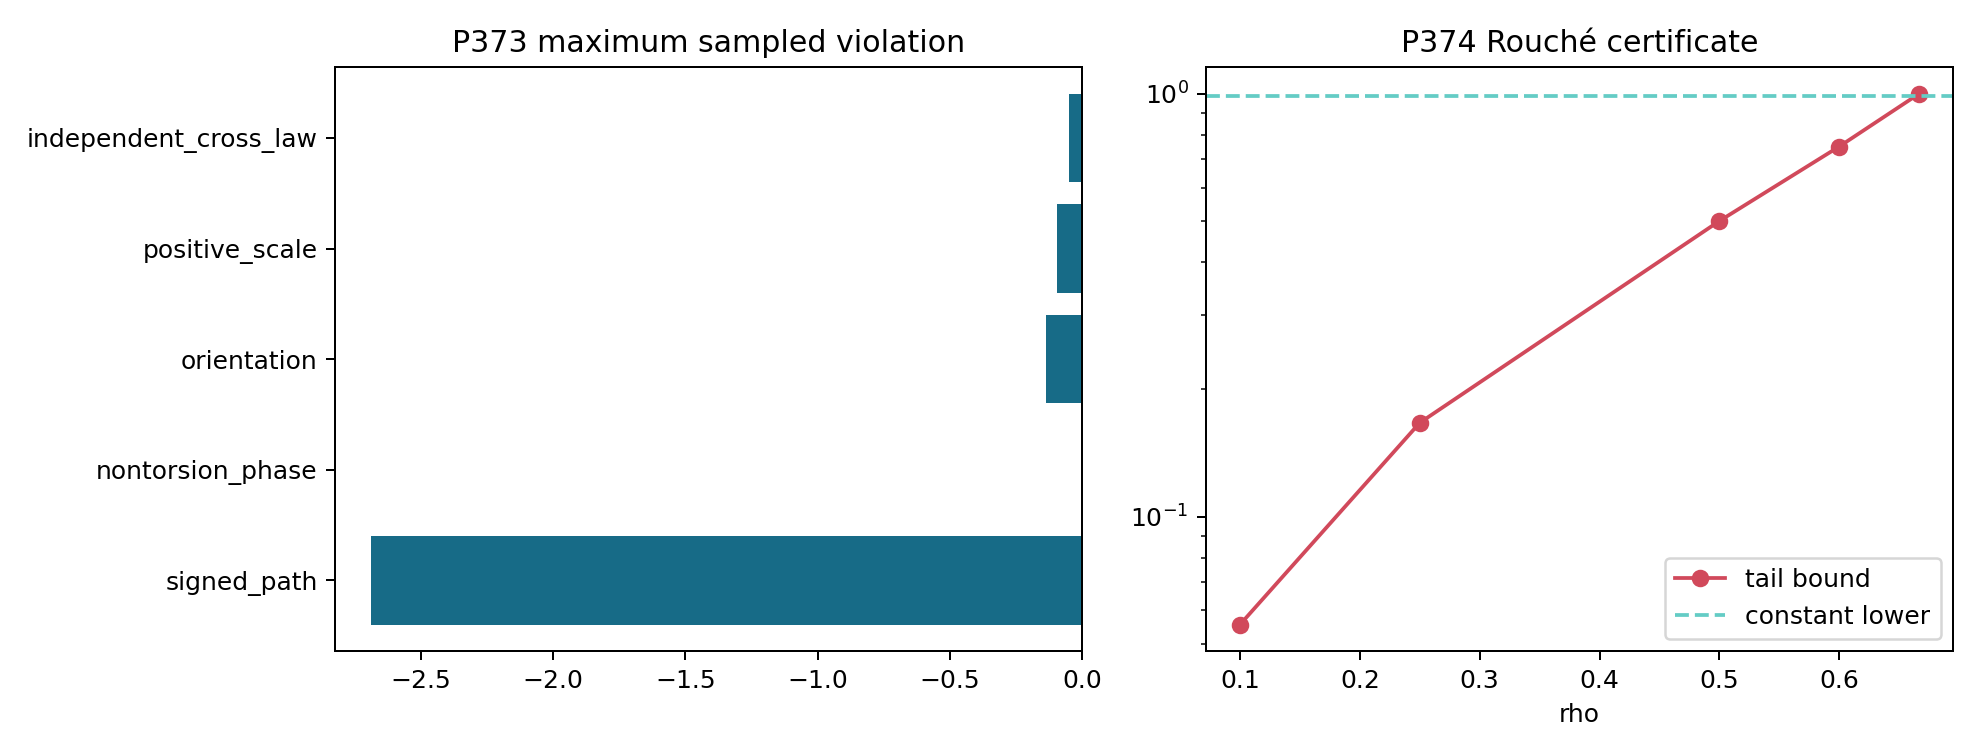
\includegraphics[width=0.97\textwidth]{FIN_Programs_365_378_Figures/p373_p374_semantics_outer.png}
\caption{Operational data-processing semantics and the noncanonical zero-free outer analytic extension domain.}
\end{figure}

\chapter{P375--P376 --- conditional sector and standards gates}

\section{Conditional electroweak package}

No independently frozen manifest contains the conditional P348 prediction, sector axioms, external data, distinct roles, and one-shot unblinding.

\textbf{P375: [Blocked by external evidence]}

No legacy physical role is transferred.

\section{Dimensional standards}

No manifest supplies traceable

\[
(\ell_*,\tau_*,\hbar_*)
\]

with a covariance hash and independent roles.

\textbf{P376: [Blocked by external evidence]}

The P362 covariance pushforward is ready to consume such a record but cannot generate it.

\chapter{P377 --- the exact universality boundary of FORC}

\section{Free resource syntax}

The FORC resource object is

\[
\mathbb N^5
\]

under addition. Let \(M\) be any commutative monoid and choose five elements

\[
m_1,\ldots,m_5\in M.
\]

There is exactly one monoid homomorphism extending those generator images:

\[
\Phi(r_1,\ldots,r_5)
=
\sum_{i=1}^{5}r_im_i.
\]

Therefore \(\mathbb N^5\) is the free commutative monoid on the five resource generators.

This proves the universal property of the A2/\allowbreak{}A4 bookkeeping skeleton.

\section{Operational nonuniqueness}

Consider the same zero resource grade:

\[
r=(0,0,0,0,0).
\]

Two operational models may assign:

\[
p_A(1)=0.25,
\qquad
p_B(1)=0.75.
\]

Their total-variation distance is

\[
\operatorname{TV}(p_A,p_B)=0.5.
\]

The resource syntax does not distinguish them.

\section{Result}

\textbf{\statusProven{}} FORC is free and universal as an abstract commutative resource syntax.

\textbf{\statusRefuted{}} FORC grades uniquely determine operational probabilities or a physical realization.

A5 is not merely an interpretation of A1--A4. It contains genuinely new empirical structure.

\chapter{P378 --- reservoir process-tomography gate}

No physical reservoir bundle contains:

\begin{itemize}
\item 
calibrated preparation maps;

\item 
environmental controls;

\item 
raw event records;

\item 
a process-tomography reconstruction;

\item 
a semigroup-versus-memory model comparison;

\item 
independent custody and frozen hashes.

\end{itemize}

\textbf{[Blocked by external evidence]}

Synthetic evaluation of \(e^{-tA}\) is not reservoir engineering.

\chapter{Newly constructed theoretical objects}

\begin{center}
\begingroup\small
\setlength{\tabcolsep}{2.5pt}
\renewcommand{\arraystretch}{1.16}
\begin{longtable}{@{}p{0.278\textwidth}p{0.194\textwidth}p{0.182\textwidth}p{0.206\textwidth}@{}}
\toprule
\textbf{Object} & \textbf{Definition} & \textbf{Resolves} & \textbf{Does not resolve} \\
\midrule
\endhead
O113 Proof-Carrying Moment Interface & Independent exact checker plus archived rational identities & Self-replay risk & Lean/\allowbreak{}Coq numerical reflection \\
O114 Seven-Atom Oscillatory Cell & Exact 12-variable Krawczyk enclosure & Improved primal upper bound & Physical meaning of signed mass \\
O115 Strict \(k\)-Distance Quotient Category & Maps preserving \(d\) modulo \(k(d)\) equality & Maximal radial naturality & Legacy-to-strict completion \\
O116 Component-Gauge Identifiability Spectrum & Singular spectrum of transfer observation maps & Complex versus intensity calibration & Global hardware identifiability \\
O117 Adaptive-Angle Budget Certificate & Matching adaptive upper and parallel lower bounds & Ideal full-comb optimum to first threshold & Lossy/\allowbreak{}uncertain-clock comb \\
O118 Operational Resource-Semantics Pentagon & Five state/\allowbreak{}channel/\allowbreak{}monotone triples & Candidate meanings of O108 coordinates & FIN encoding functors \\
O119 Damped Outer Generating Family & \(F_\rho(z)=\sum K(d)\rho^dz^d\) & Existence of an outer extension & Canonical \(\rho\) or phase source \\
O120 Free-Resource/\allowbreak{}Empirical-Realization Split & Free \(\mathbb N^5\) syntax plus probability countermodel & FORC universality boundary & Unique physical theory \\
\bottomrule
\end{longtable}
\endgroup
\end{center}

\chapter{Falsification ledger}

\section{Surviving results}

\begin{enumerate}
\item 
\textbf{\statusProven{}} A second exact implementation accepts the P351/\allowbreak{}P352 certificates.

\item 
\textbf{\statusProven{}} The P366 oscillatory enclosure is narrower on both sides.

\item 
\textbf{\statusProven{}} Radial naturality is exactly naturality on the \(k\)-distance quotient.

\item 
\textbf{\statusProven{}} On diameter at most four, the strict quotient reduces to ordinary distance.

\item 
\textbf{\statusModerate{}} Complex transfer tomography is locally identifiable in the component model.

\item 
\textbf{\statusProven{}} The ideal unrestricted adaptive optimum equals the parallel optimum through the first perfect threshold.

\item 
\textbf{\statusProven{}} Five operational data-processing monotones exist.

\item 
\textbf{\statusProven{}} A noncanonical outer analytic FIN family exists.

\item 
\textbf{\statusProven{}} FORC's resource skeleton has a free universal property.

\item 
\textbf{\statusProven{}} Resource grades do not determine operational records.

\end{enumerate}

\section{Refuted promotions}

\begin{enumerate}
\item 
Independent Python checking is not proof-assistant kernel checking.

\item 
A narrower signed cost is not a physical negativity theorem.

\item 
Kernel naturality is not arbitrary graph-homomorphism naturality.

\item 
Intensity-only calibration is not equivalent to complex transfer tomography.

\item 
P371 is not a lossy or clock-robust adaptive theorem.

\item 
Operational resource monotones are not automatically FIN encodings.

\item 
An outer embedding does not derive its own coefficients.

\item 
Free resource syntax is not unique empirical physics.

\item 
A blocked external gate is neither confirmation nor falsification.

\end{enumerate}

\chapter{Present mathematical interpretation}

The current FIN structure now separates into four precise levels:

\[
\begin{array}{c}
\text{spectral operator data}\\
\downarrow\\
\text{exact signed-resource and naturality theorems}\\
\downarrow\\
\text{conditional operational encodings}\\
\downarrow\\
\text{external calibrated realization and records}.
\end{array}
\]

The first two levels contain substantial mathematics. P371 also supplies an exact operational theorem once a particular ideal unitary comparison is declared.

The third level is not unique. P373 provides plausible data-processing semantics, while P377 proves that the abstract grades do not determine them.

The fourth level remains absent. This is the precise reason FIN is not yet a physical theory.

\chapter{Recommended Programs P379--P393}

\begin{center}
\begingroup\small
\setlength{\tabcolsep}{2.5pt}
\renewcommand{\arraystretch}{1.16}
\begin{longtable}{@{}p{0.097\textwidth}p{0.284\textwidth}p{0.296\textwidth}p{0.183\textwidth}@{}}
\toprule
\textbf{Program} & \textbf{Question} & \textbf{Deliverable} & \textbf{Probability of useful result} \\
\midrule
\endhead
P379 & Can the large rational certificates be reflected through Lean/\allowbreak{}Coq? & Small proof-certificate format and kernel-checked arithmetic & 0.85 \\
P380 & Can exact contact/\allowbreak{}alternation reduce the oscillatory gap below \(10^{-7}\)? & Certified primal-dual contact theorem & 0.75 \\
P381 & Does the strict radial law have integer-distance collisions? & Global collision classification or explicit first collision & 0.80 \\
P382 & Can one enriched naturality square relate legacy and strict kernels? & One typed completion atom or a categorical no-go & 0.55 \\
P383 & Is the 132-parameter mesh globally identifiable modulo gauges? & Global gauge quotient and multitime calibration theorem & 0.70 \\
P384 & Can a calibrated twelve-mode pilot be built? & Raw-event photonic transfer bundle & 0.40 \\
P385 & Does the adaptive-angle theorem survive loss and dephasing? & Lossy comb upper/\allowbreak{}lower bounds & 0.70 \\
P386 & How does bounded clock uncertainty deform the comb threshold? & Robust discrimination interval with nuisance clock & 0.75 \\
P387 & Can one explicit FIN resource encoding functor be constructed? & Typed state/\allowbreak{}channel realization for one O108 coordinate & 0.65 \\
P388 & Are any conversions between the five operational resources possible? & Conversion matrix, catalysts, or no-go theorems & 0.60 \\
P389 & Can semigroup or RG composition select a canonical \(\rho\)? & Canonicality theorem or scale-orbit no-go & 0.65 \\
P390 & Does QW survive an independent hold-out? & Custody-separated one-shot external test & 0.50 \\
P391 & Can clock and dimensional standards be jointly calibrated? & Traceable \((\ell_*,\tau_*,\hbar_*)\) covariance package & 0.45 \\
P392 & Can a physical reservoir realize the strict heat channel? & Process tomography with Markovian alternatives & 0.35 \\
P393 & Can the conditional electroweak vector be tested blindly? & Frozen external sector test & 0.20 \\
\bottomrule
\end{longtable}
\endgroup
\end{center}

\section{P379 --- arithmetic reflection}

Design a compact certificate containing:

\begin{itemize}
\item 
fifth-root integer brackets;

\item 
Taylor remainder parameters;

\item 
Bernstein trees;

\item 
rational inverse residuals;

\item 
Krawczyk boxes;

\item 
endpoint signs.

\end{itemize}

Lean or Coq should verify it without rerunning discovery.

\section{P380 --- exact contact geometry}

The P366 gap remains approximately

\[
7.50\times10^{-5}.
\]

Recover the exact primal and dual contact set using alternation, moment semidefinite methods, or an interval KKT system.

\section{P381 --- global distance collisions}

Classify integer pairs \(d\ne e\) satisfying

\[
K_{\mathrm{strict}}(d)=K_{\mathrm{strict}}(e).
\]

Because the law oscillates while damping, global injectivity is not expected without proof. The first collision or a certified finite collision-free range directly controls the naturality category.

\section{P382 --- one enriched bridge square}

Do not restart the generic legacy-to-strict audit. Select one typed carrier, one distance quotient, and one completion atom. Test a single commutative square:

\[
\begin{array}{ccc}
K_{\mathrm{legacy}}(G)&\longrightarrow&K_{\mathrm{strict}}(G)\\
\downarrow&&\downarrow\\
K_{\mathrm{legacy}}(H)&\longrightarrow&K_{\mathrm{strict}}(H).
\end{array}
\]

\section{P383 --- global photonic gauges}

Local Jacobian rank does not exclude distant parameter aliases. Determine the exact gauge group of component losses/\allowbreak{}phases and design the smallest multitime complex calibration making the quotient identifiable.

\section{P384 --- physical pilot}

This is an external program. Require:

\begin{itemize}
\item 
complex transfer calibration;

\item 
raw timestamps;

\item 
detector calibration;

\item 
frozen protocol;

\item 
distinct provider, registrar, and analyst;

\item 
one-shot reporting.

\end{itemize}

\section{P385 --- lossy adaptive comb}

Replace unitary calls by declared attenuation/\allowbreak{}dephasing channels. Seek:

\begin{itemize}
\item 
a contractive channel-angle upper bound;

\item 
a feasible parallel or adaptive lower construction;

\item 
a quantified gap;

\item 
a dual certificate.

\end{itemize}

\section{P386 --- robust clock-comb theorem}

For

\[
\tau(t)\in
\{\tau:\tau'>0,\ |\tau''|\leq M\},
\]

propagate the clock equivalence tube through

\[
\sin\!\left(\frac{n\Delta\tau(t)}{2}\right).
\]

Determine a guaranteed discrimination interval rather than a single uncalibrated threshold.

\section{P387 --- one realization functor}

Choose exactly one resource coordinate and construct:

\begin{itemize}
\item 
FIN source object;

\item 
operational state space;

\item 
preparation;

\item 
free channels;

\item 
instrument;

\item 
record;

\item 
monotone equality or inequality.

\end{itemize}

This is the most direct internal attempt to instantiate A5 without claiming all physics.

\section{P388 --- conversions and catalysis}

The five P373 resources have different codomains. Define typed conversion channels and determine whether any resource can generate another. A negative conversion matrix would sharpen the independence theorem; a positive entry would be a genuinely new bridge.

\section{P389 --- canonical outer scale}

Test whether composition,

\[
F_{\rho_1}\star F_{\rho_2},
\]

semigroup laws, coarse graining, or an RG fixed point select one \(\rho\). If every positive \(\rho\) remains on a scale orbit, prove the no-go.

\section{P390--P393 --- external falsification}

These programs require independent organizations and physical records. Code may validate supplied manifests but may not create their evidential status.

\section{Recommended immediate order}

\[
\boxed{
\mathrm{P379}
\longrightarrow
\mathrm{P380}
\longrightarrow
\mathrm{P381}
\longrightarrow
\mathrm{P385}
\longrightarrow
\mathrm{P387}
}.
\]

\chapter{Final conclusion}

Programs P365--P378 sharpen the theory at three distinct boundaries.

First, the signed-moment results become more trustworthy and narrower. Independent exact implementation reproduces the certificates, and a seven-atom Krawczyk cell improves the full oscillatory enclosure.

Second, two previously open mathematical questions receive exact answers. Radial naturality lives on the \(k\)-distance quotient category. Ideal adaptive unitary discrimination is completely determined through the first perfect threshold by the relative-generator spectral diameter.

Third, the distinction between resource syntax and physics becomes a theorem. Five operational monotones can be constructed, but their connection to FIN requires separate encoding maps. FORC is universal as a free \(\mathbb N^5\) resource syntax and demonstrably nonunique as an empirical realization.

The deepest surviving interpretation is therefore:

\begin{quote}\itshape
FIN is a dimensionless spectral-operator framework with exact signed resource obstructions, a well-defined carrier-naturality category, and conditional operational models. Its abstract resource syntax does not determine a unique physical realization.

\end{quote}

The smallest missing physical object remains an independently calibrated realization functor

\[
\mathcal R:
\mathsf{FINMath}
\longrightarrow
\mathsf{OperationalModel},
\]

where

\[
\begin{aligned}
\mathsf{OperationalModel}:=\{&
\text{preparations, clocks, channels, environments,}\\
&
\text{instruments, apparatus, probabilities, and records}
\}.
\end{aligned}
\]

No spectral, categorical, or resource-universality theorem can manufacture the empirical content of \(\mathcal R\). That content must be supplied and tested.

\chapter{Reproducibility}

Run:

\begin{itemize}
\item 
MPLCONFIGDIR=/\allowbreak{}tmp/\allowbreak{}mpl-fin-1032 python3 fin\_programs\_365\_378.py

\item 
MPLCONFIGDIR=/\allowbreak{}tmp/\allowbreak{}mpl-fin-1032 python3 -m unittest -v test\_fin\_programs\_365\_378.py

\end{itemize}

Expected result: 14 tests passed, zero failed. The dependency-free Lean 4.28 structural core must compile. The P365 independent checker is executed by the main program.

\chapter{Suggested citation}

\.Zuchowski, K. (2026). \emph{FIN Research Programs P365--P378: Exact Certificate Diversity, Adaptive Discrimination, Operational Resource Semantics, and the Universality Boundary} (Release 10.32; Version 1.0.0) [Preprint]. Zenodo.


\clearpage
\chapter*{Reproduction certificate}
\addcontentsline{toc}{chapter}{Reproduction certificate}
\begin{Verbatim}[fontsize=\small]
MPLCONFIGDIR=/tmp/mpl-fin-1032 \
python3 fin_programs_365_378.py

MPLCONFIGDIR=/tmp/mpl-fin-1032 \
python3 -m unittest -v test_fin_programs_365_378.py
\end{Verbatim}
Expected result: 14 tests passed, 0 failed. The dependency-free Lean 4.28
structural core must compile. P367, P370, P372, P375, P376, and P378 remain
external admission gates; no synthetic record is accepted as laboratory,
standards, hold-out, or custody evidence.

\medskip
\noindent\textbf{Suggested citation:}

\.Zuchowski, K. (2026). \emph{FIN Research Programs P365--P378:
Exact Certificate Diversity, Adaptive Discrimination, Operational Resource
Semantics, and the Universality Boundary} (Release 10.32; Version 1.0.0)
[Preprint]. Zenodo.

\end{document}
